\documentclass[sigconf,nonacm]{acmart}

\AtBeginDocument{%
  \providecommand\BibTeX{{Bib\TeX}}%
}

\settopmatter{printacmref=false}
\renewcommand\footnotetextcopyrightpermission[1]{}
\pagestyle{plain}

\usepackage{booktabs}
\usepackage{enumitem}
\usepackage{graphicx}
\usepackage{listings}
\usepackage{algorithm}
\usepackage{algpseudocode}
\usepackage{float}

\setlength{\emergencystretch}{2em}
\setlength{\textfloatsep}{8pt plus 2pt minus 2pt}
\setlength{\floatsep}{8pt plus 2pt minus 2pt}
\setlength{\dbltextfloatsep}{8pt plus 2pt minus 2pt}
\setlength{\dblfloatsep}{8pt plus 2pt minus 2pt}

\lstset{
  basicstyle=\ttfamily\footnotesize,
  breaklines=true,
  columns=fullflexible,
  frame=single,
  literate={□}{{$\square$}}1
}


\newcommand{\hole}[1]{\ensuremath{\{\square\!:\!\text{\texttt{#1}}\}}}

\title{ReSketch: Corpus-Guided Semantic Regex Synthesis}

\author{Berk Cakar}
\affiliation{%
  \department{Course Project Final Report\\ECE 663: Program Synthesis\\Spring 2026}
  \institution{Purdue University}
  \city{West Lafayette}
  \state{IN}
  \country{USA}}

\begin{document}

\begin{abstract}
Writing a correct regular expression demands low-level syntactic knowledge
that is often far removed from the user's intent.
A user may know that a field should hold an email address or a CVV code,
yet translating that knowledge into a precise pattern remains error-prone.
ReSketch addresses this gap with \emph{semantic sketches}: partial regexes
whose open positions are typed holes such as \hole{email\_address} or
\hole{cvv}.
Given a sketch and a set of positive and negative examples, ReSketch
retrieves reusable regex components for each hole, decomposes the global
examples into per-hole evidence, and searches over candidate components
and refinements to assemble a validated regex.
On a suite of nine demonstration tasks spanning single-hole, multi-hole, and
ambiguous-decomposition scenarios, the prototype solves all tasks under
default settings; a decomposition ablation shows that hole-local
evidence is necessary for multi-hole synthesis.
\end{abstract}

\maketitle

\section{Introduction}
Regular expressions are a compact notation for describing sets of strings,
widely used for validation, data extraction, log processing, and input
sanitization. Yet empirical studies find that developers struggle
to read, write, and maintain
them~\cite{michael2019regexes}. The consequences go beyond readability:
regex mistakes cause string-processing bugs and security vulnerabilities such
as Regular Expression Denial of
Service~\cite{wang2021demystifying,davis2018redos,davis2021memoization,bhuiyan2025sok}.
A user may know that a field should hold an email address, an IPv4 address, or
a payment-related token, but translating that semantic intent into a correct
pattern remains difficult.

Program synthesis can help. Instead of writing the final expression directly,
a user can supply examples, natural language, or partial specifications and let
a synthesizer search for a consistent
program. Programming-by-example has proved effective for string transformations
in spreadsheets~\cite{gulwani2011automating}, and several systems apply the
idea to regex synthesis from examples and multimodal
specifications~\cite{lee2016synthesizing,chen2020multimodal}. Semantic regex
synthesis goes one step further: practical extraction tasks often require
domain-level concepts (dates, currencies, IP addresses) that plain regex syntax
cannot express directly~\cite{chen2023data}. Examples alone, however, leave
the intended semantic category implicit. A handful of positive and negative
strings may separate one candidate regex from another, but they do not tell the
synthesizer that the user wanted a credit-card field rather than an arbitrary
digit sequence.

ReSketch introduces a different starting point: the \emph{semantic sketch}.
The user writes a partial regex with typed holes such as
\hole{email\_address} or \texttt{CVV:}\hole{cvv}, fixing the surrounding
structure while leaving semantically meaningful sub-expressions open. ReSketch
completes those holes by retrieving reusable regex components from an annotated
corpus, a language model, or both. This design reflects observed developer
practice---regexes are frequently copied and
adapted~\cite{davis2019lingua}---and is consistent with recent evidence that
both reuse and LLM-based generation are competitive strategies for regex
composition~\cite{cakar2025reuse}. Retrieval proposes candidate components;
examples remain the behavioral specification that drives decomposition,
ranking, and validation.

The resulting system is both a research vision and a course-project prototype.
The vision is a corpus-guided synthesizer backed by an annotated corpus of
semantically labeled regexes. The prototype implements the core synthesis
pipeline behind a pluggable provider interface, so retrieval can draw on
different component sources without changing the downstream algorithm.

This report makes four contributions:
\begin{enumerate}[leftmargin=*]
  \item A \emph{semantic sketch interface} for regex synthesis that combines
  typed holes with ordinary regex context.
  \item A \emph{hybrid retrieval architecture} that treats different component
  sources as interchangeable providers of regex fragments.
  \item A \emph{prototype synthesis engine} with example decomposition,
  component-guided search, scoring, validation, and interactive counterexample
  refinement.
  \item A \emph{demonstration on nine tasks} showing that the
  prototype solves single-hole and multi-hole tasks, and that example
  decomposition is critical for multi-hole assembly.
\end{enumerate}

\section{Background and Motivation}
ReSketch draws on three lines of prior work: programming by example, which
shows that users can communicate intent through concrete behaviors rather than
complete programs; semantic regex systems, which make domain-level concepts
explicit in the synthesis problem; and empirical studies of regex reuse, which
show that developers routinely adapt existing patterns instead of writing from
scratch. Together, these motivate two design choices: typed sketches should
guide component retrieval, and examples should remain the final behavioral
specification.

\subsection{Regex Synthesis from Examples}
Programming by example (PBE) is a natural fit for regex authoring: users find
it easier to supply strings that should or should not match than to describe the
complete language of the target expression.
FlashFill showed that this interaction model works for string transformations
in spreadsheets---a user gives input-output examples, and the synthesizer
searches a domain-specific language for a consistent
program~\cite{gulwani2011automating}. Regex synthesis applies the same idea
to a different output language: given positive and negative strings, find a
regex that accepts the positives and rejects the negatives.

Early systems explored different search strategies for this problem.
Bartoli et al.\ used genetic programming to evolve regexes from labeled
extraction examples~\cite{bartoli2014automatic}.
Lee et al.\ searched for simple regexes consistent with positive and negative
examples, using over- and under-approximations to prune the candidate
space~\cite{lee2016synthesizing}.
Both illustrate the central tradeoff ReSketch also faces: examples provide a
precise behavioral test, but they do not by themselves shrink the search space.

More recent systems add a second modality to reduce ambiguity. Multimodal regex
synthesis combines natural language with examples: the language describes
high-level intent, and the examples rule out incorrect
completions~\cite{chen2020multimodal}. Sketch-driven regex generation takes
this further by mapping natural language to an incomplete regex sketch that a
synthesizer then fills using examples~\cite{ye2020sketch}.
ReSketch adopts this sketch-and-examples structure but changes the source of
the sketch: instead of deriving it from natural language, the user names
semantic holes directly, and those names drive component retrieval.

\subsection{Semantic Regular Expressions}
Many extraction tasks are only partly syntactic.
A date or IPv4 address has a recognizable surface form, but categories like
\emph{business entity} or \emph{city in Indiana} require knowledge about what
the matched text denotes, not just how it looks.
Chen et al.\ formalize this observation by extending regexes with semantic
matching constructs of the form \(\{v:\tau \mid \phi\}\), where \(\tau\) names
a semantic type and \(\phi\) optionally refines it with a
predicate~\cite{chen2023data}. Their Smore system synthesizes such semantic
regexes from positive and negative examples via neural sketch generation,
decomposition, and type-directed search.

ReSketch shares the high-level insight but makes a different engineering choice.
Instead of extending the \emph{runtime} regex language with semantic
predicates, ReSketch treats semantic names as \emph{compile-time} guidance for
retrieving ordinary regex components. A hole such as \hole{email\_address}
does not ask the matcher to query a semantic oracle at match time; it asks the
synthesizer to retrieve candidate regexes whose intended meaning matches the
label, then validate the completed expression against examples.

\subsection{Why Reuse Matters}
Regex authoring in practice is seldom a blank-page problem. Developers
routinely search for, copy, and adapt existing
expressions~\cite{davis2019lingua}, because many validation and extraction
tasks recur across applications. Reuse provides strong candidate structure, but
it is not a correctness argument by itself.

ReSketch turns this observation into a controlled retrieval-and-validation
strategy. Retrieved regexes are treated as hypotheses---they may come from an
annotated corpus, a language model, or a combination---and must survive
decomposition, search, and validation before they are accepted. Recent work
suggests that both reuse and LLM-based generation are competitive approaches to
regex composition~\cite{cakar2025reuse}, which motivates a provider-agnostic
retrieval interface: the downstream synthesis algorithm is the same regardless
of where candidates originate.

\section{System Overview}
ReSketch separates retrieval from validation. Semantic labels guide retrieval
toward plausible regex components; examples decide which candidates are
behaviorally correct. Figure~\ref{fig:pipeline} shows the main workflow,
from sketch parsing through decomposition, retrieval, search, and assembly to a
validated regex with a provenance trace. Different retrieval sources share
the same candidate-set interface, so the synthesis engine ranks, refines, and
validates components uniformly regardless of their origin.

\begin{figure*}[t]
  \centering
  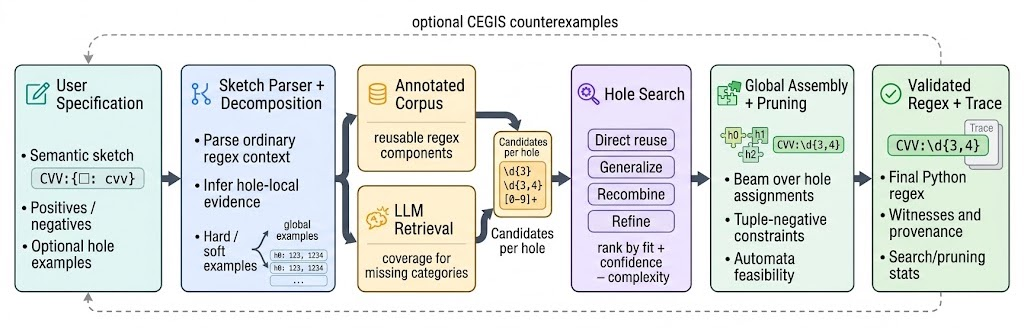
\includegraphics[width=1\textwidth,clip,trim=0 10pt 0 0]{assets/resketch_fig_1.jpg}
  \caption{Overview of ReSketch: examples decompose into hole evidence,
  candidate sources propose components, and search plus assembly produce a
  validated regex and trace.}
  \Description{A left-to-right ReSketch architecture diagram showing user
  specification, sketch parsing and decomposition, corpus and LLM retrieval,
  hole search, global assembly and pruning, and validated regex plus trace.}
  \label{fig:pipeline}
\end{figure*}

\subsection{Inputs and Outputs}
The user supplies two things: a \emph{semantic sketch}---ordinary regex context
with one or more typed holes such as \hole{email\_address}, \hole{cvv}, or
\hole{ipv4\_address}---and a set of positive and negative examples for the
complete regex. Optional hole-level examples can be added when the sketch
context does not uniquely split examples across holes.

The system returns a validated regex together with a machine-readable
\emph{trace}: retrieved candidates and their provenance, inferred per-hole
evidence, search and pruning statistics, score breakdowns, and final
validation results.

\begin{lstlisting}[caption={Example ReSketch invocation.},label={lst:cli}]
resketch synthesize \
  --sketch 'CVV:{□: cvv}' \
  --pos 'CVV:123' \
  --pos 'CVV:1234' \
  --neg 'CVV:12' \
  --neg 'CVV:abcd'
\end{lstlisting}

\subsection{Pipeline}

\paragraph{Decomposition.}
The pipeline starts by parsing the sketch into a regex AST with named holes,
preserving fixed context as structure rather than flattening it into text.
ReSketch then matches this skeleton against the global examples to infer
per-hole evidence. Unique captures become \emph{hard} local positives or
negatives; ambiguous captures become \emph{soft} evidence that influences
ranking without pruning; and some negatives produce \emph{tuple-level}
constraints that span multiple holes. Each hole's active provider then receives
the semantic type, the full sketch, and the decomposed evidence, and returns a
finite candidate set.

\paragraph{Search and assembly.}
Each hole is searched locally before global assembly. Retrieved regexes are
parsed into an internal AST when possible, then expanded through four
strategies: direct reuse, component generalization, fragment recombination, and
parameterized refinement. Candidates that violate hard local evidence are
discarded; the rest are ranked by semantic fit, source confidence, syntactic
complexity, and strategy cost. ReSketch then runs bounded beam assembly over
hole assignments, pruning partial assignments that fail global positives and
complete assignments that match global negatives. The surviving regex is
evaluated against all original examples. In interactive mode, the user can
reject a candidate and supply counterexamples; the pipeline reruns with the
strengthened specification.

\subsection{Retrieval Modes}
ReSketch treats retrieval as a pluggable provider interface. In \emph{corpus
mode}, the provider returns regex components whose labels, descriptions, or
examples match the requested semantic type. In \emph{LLM mode}, a language
model receives the semantic type, global examples, and inferred hole evidence
as prompt context and proposes candidate components. In \emph{hybrid mode},
both sources contribute to a single candidate set before search begins. This
design lets the tool operate even when one source has limited coverage for a
given category. In all modes, retrieved components are only hypotheses; they
must survive local evidence checks, global assembly, and final validation
before they are accepted.

\section{Approach}
\label{sec:approach}
The key design principle behind ReSketch is to keep semantic retrieval and
behavioral validation separate: retrieval proposes candidate components for
typed holes, but the examples and the surrounding regex context determine which
components survive. Algorithm~\ref{alg:synthesize} gives the top-level
procedure; the subsections below elaborate each step.

\begin{algorithm}[t]
\caption{\textsc{Synthesize}$(S, E^+, E^-)$}\label{alg:synthesize}
\begin{algorithmic}[1]
\Require Sketch $S$ with holes $h_1{:}\tau_1,\dots,h_k{:}\tau_k$;
         positive examples $E^+$; negative examples $E^-$
\Ensure  Validated regex $S[A]$ or failure
\Statex
\State $\mathcal{H} \gets \Call{ParseSketch}{S}$
    \Comment{extract holes and regex context}
\State $\langle L^+, \widetilde{L}^+, L^-, \mathcal{C}_{\mathrm{tn}}, \mathcal{C}_{\mathrm{rep}} \rangle
    \gets \Call{Decompose}{S, \mathcal{H}, E^+, E^-}$
    \Comment{local evidence and global constraints}
\Statex
\For{each hole $h_i \in \mathcal{H}$}
    \State $L_i \gets (L_i^+, \widetilde{L}_i^+, L_i^-)$
        \Comment{evidence for this hole}
    \State $C_i \gets \Call{Retrieve}{h_i, \tau_i, S, E^+, E^-, L_i}$
        \Comment{candidate components}
    \State $O_i \gets \emptyset$
    \For{strategy $\sigma \in \langle$\textsc{Reuse, Generalize, Recombine, Refine}$\rangle$}
        \State $O_i \gets O_i \cup \Call{BoundedSearch}_\sigma(C_i, L_i, \mathcal{C}_{\mathrm{tn}})$
    \EndFor
    \State discard options in $O_i$ that fail hard evidence $L_i^+$ or $L_i^-$
    \State rank each $o \in O_i$ by $\mathit{fit}(o) + \lambda_\rho\rho(o) - \mathit{cost}_{\mathrm{ast}}(o) - \mathit{cost}_{\mathrm{len}}(o) - \mathit{penalty}_{\sigma(o)}$
\EndFor
\Statex
\State $\mathcal{B} \gets \Call{BeamAssemble}{\{O_i\}, \mathcal{C}_{\mathrm{tn}}, \mathcal{C}_{\mathrm{rep}}, E^+, E^-}$
    \Comment{bounded beam over assignments}
\For{each assignment $A \in \mathcal{B}$}
    \If{$\forall e \in E^+.\; S[A](e)$ \textbf{and}
        $\forall e \in E^-.\; \neg S[A](e)$}
        \State \Return $S[A]$ with provenance trace
    \EndIf
\EndFor
\State \Return failure
\end{algorithmic}
\end{algorithm}

\subsection{Semantic Sketches}
A semantic sketch is a partial regex that mixes ordinary regex structure with
typed holes. Formally, we write a hole as \(h_i:\tau_i\), where \(h_i\) is a
fresh hole identifier and \(\tau_i\) is an open-vocabulary semantic label such
as \texttt{email\_address}, \texttt{cvv}, or \texttt{ipv4\_address}. A sketch
therefore has the shape of a regular expression with selected subexpressions
left unspecified:
\[
  S ::= r \mid S_1\,S_2 \mid (S_1 \;|\; S_2) \mid S^{m,n}
  \mid \{\square:\tau\}.
\]
Here \(r\) ranges over concrete regex fragments supported by the implementation,
including literals, character classes, regex categories such as \texttt{\textbackslash d},
anchors, alternation, and repetition.

Given a sketch \(S\), examples \(E^+\) and \(E^-\), and a retrieval provider
\(P\), synthesis searches for an assignment \(A\) from each hole \(h_i\) to a regex \(r_i\). Rendering the sketch with this assignment yields
\(S[A]\). A solution must satisfy the global examples:
\[
  \forall e \in E^+.~S[A](e)
  \qquad\text{and}\qquad
  \forall e \in E^-.~\neg S[A](e).
\]
The semantic type \(\tau_i\) does not change regex matching semantics at run
time; it constrains retrieval at synthesis time by asking the provider for a
finite candidate set \(C_i = P(S,h_i,\tau_i,E^+,E^-,L_i)\), where \(L_i\)
summarizes any hole-local evidence inferred from decomposition. This follows the
sketching tradition of leaving selected program fragments open while preserving
the programmer's surrounding structure~\cite{solar2008sketching,solar2006combinatorial}.
In ReSketch, that surrounding structure is itself valuable evidence: fixed
prefixes, separators, labels, and repeated contexts help decompose global
examples into constraints on individual holes.

\subsection{Hybrid Candidate Retrieval}
For each hole \(h_i:\tau_i\), ReSketch constructs a retrieval request containing
the semantic type, the full sketch, the global examples, and any hole-local
evidence inferred from decomposition. A provider returns a bounded set of
components
\[
  C_i = \{(r, d, \rho, W_r^+, W_r^-, s)\},
\]
where \(r\) is a regex fragment, \(d\) is a short description, \(\rho\) is an
optional confidence score, \(W_r^+\) and \(W_r^-\) are positive and negative
witness strings supplied with the component, and \(s\) records provenance.
The notation \(E^+\) and \(E^-\) is reserved for the user's global examples.
ReSketch uses this common schema for all retrieval sources, so the later
synthesis stages do not depend on whether a component came from an annotated
corpus, an LLM, or both.

\paragraph{Corpus retrieval} returns components that have already been labeled
with semantic intent. A request for \texttt{cvv} or \texttt{zip\_code}
retrieves components whose annotations, descriptions, or examples match that
category.
\paragraph{LLM retrieval} treats a language model as an open-vocabulary
component proposer: it receives the same request context and returns candidate
regexes with descriptions, confidence values, and example witnesses. This
follows a broader synthesis pattern in which informal signals propose likely
program fragments while examples supply behavioral
constraints~\cite{rahmani2021multimodal,chen2020multimodal}.
\paragraph{Hybrid retrieval} unions the candidate sets from the enabled
sources, deduplicates equivalent regex strings, and preserves source
provenance. The goal is not to trust more components but to give search a
diverse frontier: corpus retrieval can supply stable reusable idioms, while LLM
retrieval can cover labels that are sparse or absent from the
corpus~\cite{cakar2025reuse}. Regardless of origin, all candidates pass
through the same local checks, transformations, and global validation.

\subsection{Example Decomposition}
Global examples describe the whole regex, but hole search benefits from local
evidence. ReSketch derives this evidence by interpreting the sketch as a partial
matcher: concrete regex structure is matched normally, while each hole captures
a bounded substring. For a positive example \(e \in E^+\), the matcher
enumerates capture assignments
\[
  \mathcal{A}(e) = \{\alpha \mid S[\alpha]\text{ is consistent with }e\}.
\]

\paragraph{Hard and soft evidence.}
If all assignments agree that hole \(h_i\) captured value \(v\), ReSketch
records \(v\) as \emph{hard} positive evidence \(L_i^+\). For example,
\texttt{CVV:123} decomposes uniquely against \texttt{CVV:}\hole{cvv}, yielding
\texttt{123} as a local witness. When several splits are possible---adjacent
holes or ambiguous alternations---the captures are recorded as \emph{soft}
positives \(\widetilde{L}_i^+\). Soft evidence improves ranking but does not
prune candidates on its own.

\paragraph{Negative decomposition.}
Negatives are decomposed conservatively. A unique single-hole capture becomes
hard negative evidence \(L_i^-\). A unique multi-hole capture becomes a
\emph{tuple-negative constraint}: each value may be reasonable alone, but the
joint assignment must be rejected during global assembly. Repeated occurrences
of the same hole produce consistency constraints over the captured values.
Decomposition thus converts the sketch's fixed regex context into pruning
information without requiring manual hole-level labels.

\subsection{Component-Guided Search}
For each hole, ReSketch turns retrieved components into a local search frontier.
Components that are syntactically invalid or too large are discarded; the rest
are parsed into an internal regex AST so that the synthesizer can manipulate
regex structure rather than raw strings. Search then produces a ranked option
set \(O_i\) for hole \(h_i\), using four strategies in increasing order of
flexibility.

\emph{Direct reuse} keeps a retrieved component unchanged. This is the cheapest
strategy and captures the case where a provider already proposed the right
regex. \emph{Component generalization} combines pairs of retrieved components by
anti-unification: for instance, compatible character classes can be widened,
literal positions can be generalized to classes, and nearby repetitions can be
merged into a broader quantifier. \emph{Fragment recombination} extracts
subexpressions from retrieved components and hole examples, then enumerates
small expressions built with concatenation, alternation, optionality, and
bounded repetition. Finally, \emph{parameterized refinement} makes local edits to
promising components, such as adjusting repeat bounds, swapping character
classes, toggling anchors, or inserting optional separators suggested by the
examples.

Every generated candidate is normalized, rendered back to a regex, and checked against the hard local evidence \(L_i^+\) and \(L_i^-\).
Candidates that fail hard evidence are pruned. Soft positives
\(\widetilde{L}_i^+\) and tuple-negative probes affect the score, but do not by
themselves prove correctness. To keep the search finite, ReSketch bounds AST
size, generated candidates, behavior classes, and per-hole time. It also
deduplicates both syntactically identical regexes and candidates that behave the
same on the observed local examples. The output of this phase is therefore not a
single regex per hole, but a compact set of diverse, evidence-compatible options
for global assembly.

\subsection{Ranking, Validation, and CEGIS}
Each hole option receives a score that balances behavioral evidence and
simplicity:
\[
  \mathit{score}(o)=
  \mathit{fit}(o)+\lambda_\rho\rho(o)
  -\mathit{cost}_{\mathrm{ast}}(o)-\mathit{cost}_{\mathrm{len}}(o)
  -\mathit{penalty}_{\mathrm{strategy}}(o).
\]
The fit term rewards hard local matches, hard local rejections, soft positive
matches, and tuple-negative probe rejections. Source confidence \(\rho(o)\)
lets retrieval sources express uncertainty, while syntactic cost and strategy
penalties prefer smaller regexes and more direct explanations when examples do
not distinguish alternatives.

\paragraph{Global assembly.}
Assembly searches over assignments \(A\) that choose one option from each
\(O_i\). ReSketch orders holes by available evidence and constraint
participation, then runs bounded beam search over partial assignments.
Tuple-negative and repeated-hole constraints prune assignments before a full
regex is rendered. When automata-backed pruning applies, partial assignments are
checked for positive-example feasibility and complete assignments for
negative-example rejection; otherwise the engine falls back to regex-based
validation. Surviving assignments are rendered as \(S[A]\) and evaluated
against the original \(E^+\) and \(E^-\).

\paragraph{Interactive refinement (CEGIS).}
In interactive mode, each synthesis round ends with a user decision: accept the
candidate regex or reject it by supplying new positive or negative
counterexamples. Counterexamples are appended to \(E^+\) or \(E^-\), and the
full pipeline reruns under the strengthened specification. This follows the
standard CEGIS pattern of alternating synthesis with concrete counterexamples
to refine an incomplete specification~\cite{jha2017theory}.

\begin{table*}[t]
  \caption{Demonstration task specifications. Each task has 1--3 positive and 1--3
    negative examples; one of each is shown. Multi-hole sketches are abbreviated
    for readability.}
  \label{tab:task-specs}
  \centering
  \scriptsize
  \begin{tabular*}{\textwidth}{@{\extracolsep{\fill}}lclll@{}}
    \toprule
    Task & \#$E^+$/\#$E^-$ & Sketch & Positive example & Negative example \\
    \midrule
    email-address & 2/2 &
      \hole{email\_address} &
      \texttt{john.doe@example.com} &
      \texttt{missing-at.example.com} \\
    signed-integer & 3/2 &
      \hole{integer} &
      \texttt{-42} &
      \texttt{3.14} \\
    cvv-after-label & 2/2 &
      \texttt{CVV:}\hole{cvv} &
      \texttt{CVV:123} &
      \texttt{CVV:12} \\
    payment-receipt & 2/2 &
      \texttt{CARD:}\hole{credit\_card}\texttt{ EXP:}\hole{exp\_date} \ldots &
      \texttt{CARD:4111\,\ldots\,EXP:04/26 CVV:123 AMT:\$19.95} &
      \texttt{\ldots\,EXP:13/26\,\ldots} \\
    server-log & 2/2 &
      \hole{iso\_date}\texttt{ }\hole{ipv4}\texttt{ "}\hole{method}\texttt{ }\hole{path}\texttt{"} &
      \texttt{2026-04-27 192.168.0.1 "GET /api/v1/orders"} &
      \texttt{\ldots\,"BLAH /api/v1/orders"} \\
    product-code & 2/3 &
      \hole{product\_code} &
      \texttt{A12},\;\texttt{AB12} &
      \texttt{A13},\;\texttt{B12} \\
    ambiguous-split & 2/3 &
      \hole{alpha}\hole{integer} &
      \texttt{AB123} &
      \texttt{123AB} \\
    nested-repeat & 2/3 &
      \texttt{IDS:(?:}\hole{integer}\texttt{-)\{2\}}\hole{integer} &
      \texttt{IDS:12-34-56} &
      \texttt{IDS:12-34} \\
    tuple-negative & 1/1 &
      \hole{year}\texttt{-}\hole{integer} &
      \texttt{2026-42} &
      \texttt{3026-42} \\
    \bottomrule
  \end{tabular*}
\end{table*}

\section{Prototype Implementation}
The prototype is a Python~3.11 command-line tool built around the provider
interface and synthesis engine described above. It is a working demonstration
of the full ReSketch pipeline.

\subsection{Command-Line Tool}
The tool exposes a CLI. The main
command, \texttt{resketch synthesize}, accepts a sketch, positive and negative
examples, a retrieval mode, and synthesis controls (beam size, decomposition
mode, automata pruning). Auxiliary commands validate an existing regex, inspect
parsed holes, print the resolved configuration, and run a small task suite.

\subsection{Synthesis Engine}
The engine parses sketches into an AST with explicit hole nodes, rejects
unsupported non-regular constructs, and uses Python regex semantics for
candidate validation. It handles embedding details such as stripping outer
anchors when a retrieved component is inserted inside a larger sketch.
Automata-backed pruning is implemented for the supported fullmatch subset and
fails open to regex-based checks when a construct falls outside that subset.

\paragraph{Auditability.}
Every synthesis result carries enough metadata to make decisions auditable:
the trace records retrieved candidates with provenance, inferred per-hole
evidence, search and pruning statistics, score breakdowns, and validation
outcomes. The interactive runner wraps the synthesizer in the CEGIS loop
described in Section~\ref{sec:approach}: a rejected candidate can be refined
by adding counterexamples, after which the pipeline reruns.

\subsection{Retrieval Provider Boundary}
The current prototype separates retrieval from synthesis through a common
candidate-provider schema. This is the mechanism that lets ReSketch treat
different component sources as interchangeable: each provider receives the
same request context and returns candidates in the same format. The downstream
synthesis algorithm does not depend on which provider produced a candidate;
once candidates are returned, all sources are normalized, searched, ranked,
and validated through the same pipeline. Details about collecting and
characterizing reusable regex components are outside this report's
implementation focus and are deferred to the reuse
study~\cite{cakar2025reuse}.

\section{Demonstration}
We tested the prototype on nine synthesis tasks
(Table~\ref{tab:task-specs}) covering single-hole reuse, labeled-context
decomposition, multi-hole beam assembly, ambiguous adjacent holes, repeated
holes under quantifiers, and tuple-negative constraints.
Table~\ref{tab:demo-results} summarizes the results: under this configuration,
ReSketch solves all nine tasks.

\subsection{Task Suite}
The suite spans three complexity levels. Three \emph{single-hole} tasks
(email-address, signed-integer, cvv-after-label) test direct reuse of
retrieved components. Two \emph{four-hole} tasks (payment-receipt, server-log)
test beam assembly: the payment receipt assembles credit-card, expiration-date,
CVV, and currency-amount components into one regex, while the server log
requires a fragment-recombination step for the HTTP method hole because neither
positive method alone covers both examples. Four remaining tasks target
specific engine behaviors: ambiguous adjacent holes, a repeated hole under a
quantifier, a tuple-negative constraint, and component generalization from
concrete examples.

Representative synthesized regexes include
\texttt{CVV:\textbackslash d\{3,4\}} for the labeled CVV task,
\texttt{[A-Z]\{1,2\}\textbackslash d+} for the ambiguous split, and
\texttt{20\textbackslash d\{2\}-\textbackslash d+} for the
tuple-negative task, where the year component narrows from a four-digit
pattern to a 2000s-range pattern to reject the negative \texttt{3026-42}.

\subsection{Metrics}
The ``Cands'' column in Table~\ref{tab:demo-results} reports the total number
of local candidates evaluated across all holes. Even direct-reuse outcomes can
evaluate hundreds of candidates because each retrieved component seeds bounded
generalization, recombination, and refinement. Tasks with one or two holes
explore 600--1\,800 candidates; four-hole tasks explore 3\,600--3\,900 because
each hole contributes its own search frontier. ``Len'' shows the character length
of the synthesized regex, ranging from 11 for simple single-hole tasks to 86
for the four-hole server log. Decomposition achieves 100\% hard-evidence
coverage on all tasks except ambiguous-split, whose two adjacent holes produce
only soft evidence: the trace records 16 soft positives and 2 ambiguity
groups, showing that the engine distinguishes unique from
ambiguous captures.

\begin{table}[!ht]
  \caption{Demonstration results on nine tasks. All tasks
    solved successfully in this run. \#H = number of
    typed holes; Len = synthesized regex length in characters.
    Strategies: DR = direct reuse,
    FR = fragment recombination, PR = parameterized refinement.}
  \label{tab:demo-results}
  \centering
  \footnotesize
  \begin{tabular*}{\columnwidth}{@{\extracolsep{\fill}}lrrrl@{}}
    \toprule
    Task & \#H & Cands & Len & Strategies \\
    \midrule
    email-address     & 1 & 1\,148 & 50 & DR \\
    signed-integer    & 1 &   808  & 11 & DR \\
    cvv-after-label   & 1 &   703  & 11 & DR \\
    payment-receipt   & 4 & 3\,600 & 82 & DR, PR \\
    server-log        & 4 & 3\,878 & 86 & DR, FR \\
    product-code      & 1 &   615  & 11 & DR \\
    ambiguous-split   & 2 & 1\,660 & 13 & DR \\
    nested-repeat     & 1 & 1\,749 & 19 & DR \\
    tuple-negative    & 2 & 1\,636 & 12 & DR \\
    \bottomrule
  \end{tabular*}
\end{table}

\subsection{Walkthrough: Request-Log Task}
To show the pipeline stages concretely, we trace a five-hole task whose sketch
mixes literal regex context with typed holes:

\begin{lstlisting}
\[{□: iso_date}T{□: time}\]
  req={□: alpha}{□: integer}
  status={□: status_code}
\end{lstlisting}

\noindent Two positive examples and two negatives are supplied:
\begin{lstlisting}
pos: [2026-04-27T14:05:33] req=AB123 status=200
pos: [2026-01-15T08:30:00] req=CD456 status=201
neg: [2026-04-27T14:05:33] req=123AB status=200
neg: [2026-04-27T14:05:33] req=AB123 status=999
\end{lstlisting}

\paragraph{Decomposition.}
ReSketch matches the sketch skeleton against each positive example and extracts
per-hole captures. The brackets and literal labels \texttt{T}, \texttt{req=},
and \texttt{status=} act as unambiguous separators, so three holes receive
hard positive evidence: \texttt{iso\_date} captures \texttt{2026-04-27} and
\texttt{2026-01-15}, \texttt{time} captures \texttt{14:05:33} and
\texttt{08:30:00}, and \texttt{status\_code} captures \texttt{200} and
\texttt{201}. The two adjacent holes \texttt{alpha} and \texttt{integer} have
no separator, so the boundary is ambiguous: the string \texttt{AB123} can be
split as (\texttt{A},\texttt{B123}), (\texttt{AB},\texttt{123}),
(\texttt{AB1},\texttt{23}), and so on. ReSketch records all possible splits as
soft positive evidence and marks two ambiguity groups.

\paragraph{Retrieval and search.}
In this run, candidate retrieval returns 5--8 regex components per hole from the active
provider. Search explores all four strategies: direct reuse tries each
retrieved component unchanged; fragment recombination builds small expressions
from sub-fragments; parameterized refinement adjusts quantifier bounds and
character classes; and component generalization attempts anti-unification of
component pairs. The three hard-evidence holes prune most generated candidates
quickly: for instance, \texttt{iso\_date} generates 1\,194 candidates, of
which 1\,158 are discarded because they fail the hard local examples. The two
soft-evidence holes (\texttt{alpha} and \texttt{integer}) have no hard
constraints to prune against, so generated candidates are not pruned by hard
local evidence and are instead ranked by soft-evidence fit and syntactic cost.

\paragraph{Scoring and assembly.}
For each hole, surviving candidates are scored by semantic fit, source
confidence, AST complexity cost, and strategy penalty. For the
\texttt{status\_code} hole, a fragment \texttt{\textbackslash d*}
(score~5.7) scores slightly above a retrieved component
\texttt{[1-5][0-9]\{2\}} (score~5.5) in per-hole ranking, but during beam
assembly the broader fragment is eliminated because it accepts the negative
status \texttt{999}. The range-restricted component survives global
validation and is selected. Beam assembly combines per-hole options into
global assignments, checking each complete assignment against all four
examples. The
validated output is:

\begin{lstlisting}
\[[0-9]{4}\-[0-1][0-9]\-[0-3][0-9]T\d{2}:\d{2}:\d{2}\]
  req=\w*\d+ status=[1-5][0-9]{2}
\end{lstlisting}

\noindent The provenance trace records that three holes were filled by direct
reuse with anchor stripping, while the \texttt{alpha} hole was filled by
fragment recombination since no single retrieved component matched the
ambiguous soft evidence.

\subsection{Decomposition Ablation}
To measure how much example decomposition contributes, we reran four tasks
under three decomposition modes: the default hard-and-soft mode, hard-only
mode (soft evidence is not used for ranking), and decomposition disabled
entirely. Table~\ref{tab:ablation} shows the results.

\paragraph{Without decomposition,} three of four tasks fail outright. The
survivor, ambiguous-split, produces a narrower regex
(\texttt{[A-Z]\{2\}\textbackslash d\{3\}}) that overfits to the two positive
examples instead of generalizing.

\begin{table}[H]
  \caption{Decomposition ablation on four tasks.  Each cell shows the
    number of candidates explored; \textsf{F} marks a failed synthesis.}
  \label{tab:ablation}
  \centering
  \footnotesize
  \begin{tabular*}{\columnwidth}{@{\extracolsep{\fill}}lrrr@{}}
    \toprule
    Task & Default & No decomp & Hard-only \\
    \midrule
    payment-receipt  & 3\,600  & \textsf{F} & 3\,600 \\
    server-log       & 3\,878  & \textsf{F} & 3\,878 \\
    ambiguous-split  & 1\,660  &   617      &   619  \\
    product-code     &   615   & \textsf{F} &   615  \\
    \bottomrule
  \end{tabular*}
\end{table}

\paragraph{Hard-only mode} does not change the outcome on tasks whose
decomposition is unambiguous, but it reduces the candidate count on
ambiguous-split from 1\,660 to 619 and yields a slightly less general regex
(\texttt{[A-Z]\{2\}\textbackslash d+} instead of
\texttt{[A-Z]\{1,2\}\textbackslash d+}), because soft evidence no longer
guides search toward broader candidates.

These results show that decomposition is necessary for the multi-hole tasks in
this suite, and that soft evidence can improve generalization when hard
decomposition is ambiguous.

\section{Limitations and Future Work}
Three limitations bound the claims above.

\paragraph{Bounded search.}
AST size, candidate counts, behavior classes, and per-hole time are all capped
by configuration. Completeness holds only within these bounds; the engine
reports its completeness status in the trace so that users can tell whether
search was exhaustive or truncated.

\paragraph{Regex subset.}
The supported subset excludes lookahead, lookbehind, backreferences, and other
non-regular constructs. Sketches or candidates that use these features are
rejected or treated as raw regexes only when raw-regex handling is enabled; in
either case, they fall outside AST-level manipulation and automata pruning.

\paragraph{Retrieval nondeterminism.}
When the retrieval source is nondeterministic, the set of candidates explored
can differ across runs. Validation catches candidates that fail the current
examples, but two runs on the same specification may still produce different
regexes that satisfy those examples.

Three directions would strengthen the system. First, the annotated component
corpus should be expanded to improve coverage of common categories. Second,
larger comparisons against existing regex synthesizers and direct LLM
generation would clarify where corpus-guided synthesis adds value. Third,
learned ranking from synthesis outcomes could replace the current fixed scoring
weights.

\section{Conclusion}
ReSketch shows that semantic sketches and reusable regex components can make
regex synthesis more structured: the user names what each hole should mean,
and the system turns that intent into a validated regex through decomposition,
search, and example-driven validation. The demonstration on nine tasks shows
that the prototype handles both single-hole and multi-hole synthesis under the
tested configuration. The decomposition ablation further shows that
hole-local evidence is important for the multi-hole tasks in this suite. The
prototype is a course-project artifact with clear limitations, but it
implements a working path from sketch to validated regex and provides a
concrete foundation for future work.

\section*{Data Availability}
The ReSketch prototype, benchmark tasks, and demonstration scripts are
available at \url{https://github.com/friberk/ReSketch}.

\bibliographystyle{ACM-Reference-Format}
\bibliography{resketch-references}

\end{document}
